% این تمپلیت از درس ساختمان داده ی دکتر علیمی-پاییز۹۹ برداشته شده است.

\documentclass[11pt]{article}
\usepackage{pgfplots}

\usepackage{tikz}
\usetikzlibrary{datavisualization}
\usetikzlibrary{datavisualization.formats.functions}


%You should edit HW.tex, not this file!
\usepackage{mathtools, amsmath, nccmath}
\usepackage{bm}
\usepackage{amsthm}
\usepackage{latexsym}
\usepackage{amssymb}
\usepackage{verbatim}
\usepackage{enumitem,array}
\usepackage{tikz}
\usepackage{color}
\usepackage{bookmark}
\usepackage{geometry}
\geometry{
 a4paper,
 right=15mm,
 left=15mm,
 top = 10mm,
 bottom = 20mm
}
\usepackage{listings}
\usepackage{bussproofs} %for prooftrees
\usepackage{hyperref}
\hypersetup{
	colorlinks=true,
	linkcolor=blue,
	filecolor=magenta,      
	urlcolor=cyan,
}
\usepackage{xepersian}

\definecolor{light-gray}{gray}{0.98}
\definecolor{blue-green}{rgb}{0,0.6,0.5}
\lstset{ 
  backgroundcolor=\color{light-gray},   % choose the background color; you must add \usepackage{color} or \usepackage{xcolor}; should come as last argument
  basicstyle=\footnotesize\color{violet},        % the size of the fonts that are used for the code
  breakatwhitespace=false,         % sets if automatic breaks should only happen at whitespace
  breaklines=true,                 % sets automatic line breaking
  %frame=lines
  captionpos=b,                    % sets the caption-position to bottom
  commentstyle=\itshape\color{blue-green},    % comment style
  %escapeinside={\%*}{*)},          % if you want to add LaTeX within your code
  extendedchars=true,              % lets you use non-ASCII characters; for 8-bits encodings only, does not work with UTF-8
  frame=single,	                   % adds a frame around the code
  keepspaces=true,                 % keeps spaces in text, useful for keeping indentation of code (possibly needs columns=flexible)
  keywordstyle=\bfseries\color{blue},       % keyword style
  %language=Octave,                 % the language of the code
  morekeywords={*,...},            % if you want to add more keywords to the set
  numbers=left,                    % where to put the line-numbers; possible values are (none, left, right)
  numbersep=5pt,                   % how far the line-numbers are from the code
  numberstyle=\tiny\color{gray}, % the style that is used for the line-numbers
  rulecolor=\color{light-gray},         % if not set, the frame-color may be changed on line-breaks within not-black text (e.g. comments (green here))
  showspaces=false,                % show spaces everywhere adding particular underscores; it overrides 'showstringspaces'
  showstringspaces=false,          % underline spaces within strings only
  showtabs=false,                  % show tabs within strings adding particular underscores
  stepnumber=1,                    % the step between two line-numbers. If it's 1, each line will be numbered
  stringstyle=\color{cyan},     % string literal style
  tabsize=2,	                   % sets default tabsize to 2 spaces
  %title=\lstname                   % show the filename of files included with \lstinputlisting; also try caption instead of title
}
%\setlist[enumerate,1]{start=0} %for 0-based enumeration

%\settextfont[
 %BoldFont={HM_XNiloofarBd.ttf}, 
 %ItalicFont={HM_XNiloofarIt.ttf},
 %BoldItalicFont={HM_XNiloofarBdIt.ttf}
 %]{HM_XNiloofar.ttf}
\settextfont{HM XNiloofar}
\ExplSyntaxOn \cs_set_eq:NN \etex_iffontchar:D \tex_iffontchar:D \ExplSyntaxOff
\setdigitfont{HM XNiloofar}
%\setdigitfont{ParsiDigits}
\defpersianfont\outline[Scale=1]{HM XNiloofar Outline}
\setlength{\parindent}{1.5em}
\setlength{\parskip}{0.9em}
\renewcommand{\baselinestretch}{1.5}

%for persian enumeration
\makeatletter
\def\@myharfi#1{\ifcase#1\or آ\or ب\or پ\or ت\or ث\or
ج\or چ\or ح\or خ\or د\or ذ\or ر\or ز\or س\or ش\or ص\or ض\or ع\or غ\or
ف\or ق\or ک\or گ\or ل\or م\or ن\or و\or ه\or ی\else\@ctrerr\fi}
\def\myharfi#1{\expandafter\@myharfi\csname c@#1\endcsname}
\makeatother
\AddEnumerateCounter{\myharfi}{\@myharfi}{}

\newcommand{\lecture}[4]{
%\pagestyle{empty}

	%\begin{center}
	%		\vspace{-1cm}
	%	   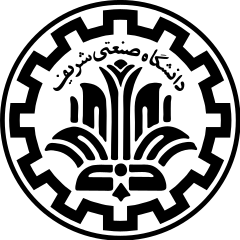
\includegraphics[scale=0.15]{Sharif}%\hfill \\[1em]  
	%\end{center}
	%\vspace{-3em}
\begin{center}

\bf
%\begin{outline} 
{
\LARGE
#1
}
%\end{outline} 
\\
تمرین #2
\end{center}
\vspace*{-1em}
\noindent
نام و نام‌خانوادگی: #3 \hfill شماره دانشجویی: #4
\vspace{-4mm}
\rule{\textwidth}{1pt}
%\ \\
}

% example environment
\newenvironment{example}
{\smallskip \noindent \emph{مثال:}}
{\hfill $\boxtimes$ \smallskip}

\def\Max{\text{بیشینه کن}}
\def\Min{\text{کمینه کن}}
\def\st{\text{\rl{که}}}

\newtheorem{theorem}{قضیه}
\newtheorem{proposition}{گزاره}
\newtheorem*{claim}{ادعا}
\newtheorem*{lemma}{لم}
\newtheorem{numlemma}{لم}
\newtheorem{corollary}{نتیجه}
\newtheorem*{definition}{تعریف} % Use this for non-trivial definitions.
 %%%%%%%%%%%%%%%%%%%%%%%%%%%%%%%%%%%%%%%%%%%%%%%%%%%%%%%%%%%%%%%%%%%%%%%%%%%%




\begin{document}
\lecture{1}{عنوان جلسه}{آئیریا محمدی}

می‌خواهیم 
heap
درست کنیم
.
به این شکل عمل می‌کنیم که برای هر عضو تابعی را فرا می‌خوانیم که خاصیت 
heap 
را برای آن برقرار می‌کند.
 بنا بر استقرا 
\proof
برهان خلف

فرض کنیم این‌گونه نباشد. یعنی بتوان نزدیک‌ترین عنصر آرایه 
$n$
عضوی 
$A$
به مقدار 
$x$
را در زمان 
$o(logn)$
٫ مثلا 
$O(1)$
پیدا کرد
.

آن‌گاه می‌توان الگوریتم زیر را برای مرتب کردن اعداد ارائه داد:
\lr{
\begin{codebox}
	\Procname{$\proc{sort}(A, n)$}
	\li list : LinkedList
	\li it = list.iterator : ListIterator
	\li list.add(A[0], it)  \Comment adds item to the list where iterator points, and iterator moves forward
	\li \For element 
\end{codebox}
}


مروری کوتاه بر آن‌چه گذشت و مقدمه‌ای کوتاه بر مطالب این جلسه. 

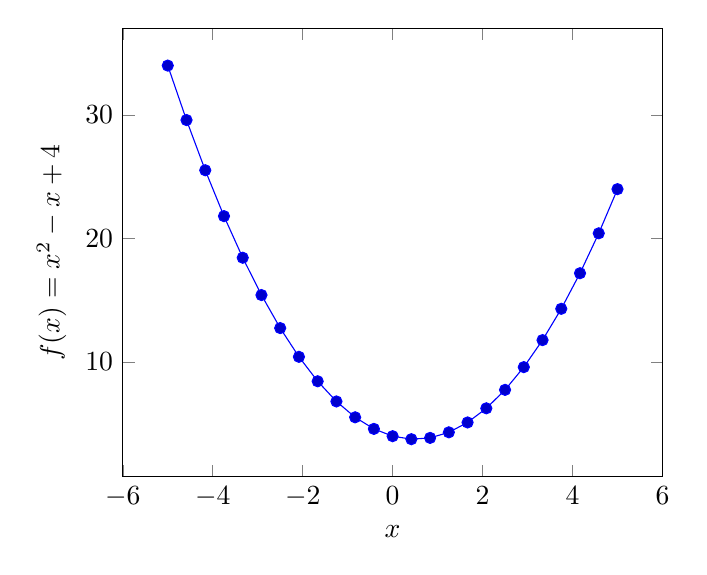
\begin{tikzpicture}
  \begin{axis}[ 
    xlabel=$x$,
    ylabel={$f(x) = x^2 - x +4$}
  ] 
    \addplot {x^2 - x +4}; 
  \end{axis}
\end{tikzpicture}

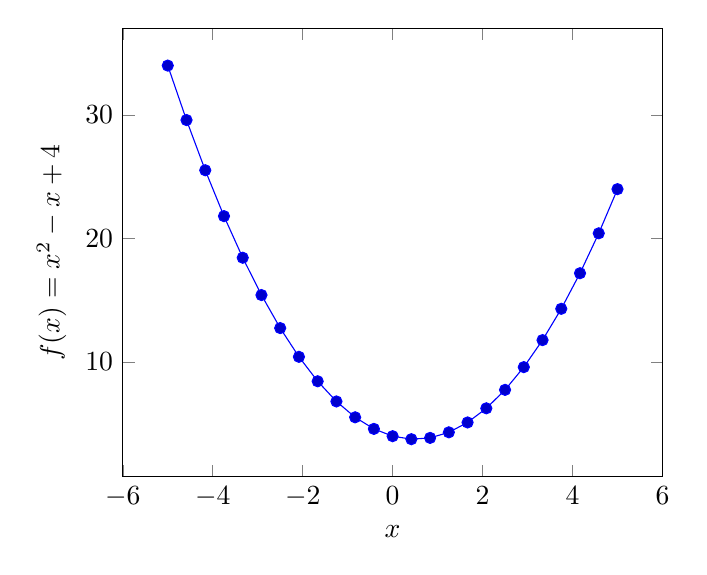
\begin{tikzpicture}
  \begin{axis}[ 
    xlabel=$x$,
    ylabel={$f(x) = x^2 - x +4$}
  ] 
    \addplot {x^2 - x +4}; 
  \end{axis}
\end{tikzpicture}

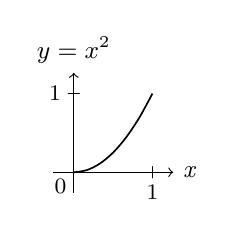
\begin{tikzpicture}
\datavisualization [school book axes,
                    visualize as smooth line,
                    y axis={label={$y=x^2$}},
                    x axis={label} ]

data [format=function] {
      var x : interval [0:1] samples 7;
      func y = \value x*\value x;
      };
\end{tikzpicture}

\section{عنوان بخش}
شروع بحث جلسه فعلی. 

پاراگراف‌ها با یک خط خالی از هم جدا می‌شوند. لازم نیست بین هر دو پاراگراف از \verb|\par|  استفاده کنیم.

می‌توانید برای نوشتن فرمول چندخطی می‌توانید از محیط \verb|align| استفاده کنید:
\begin{align*} 
\min \quad \| f \|_{\infty}\\ 
f \in F_{s,t} 
\end{align*}

سعی کنید قواعد نگارش فارسی را رعایت کنید. از نیم‌فاصله
به درستی استفاده کنید. علامت نقل قول در فارسی بدین صورت است «». پس از نقطه و ویرگول و دونقطه و پرانتزبسته‌ای که قبل از نقطه نیست و این‌گونه علامت‌ها، یک فاصله بگذارید.

خوب است معادل انگلیسی اصطلاحات را در پاورقی%
\LTRfootnote{footnote}
بیاورید.

برای نوشتن انگلیسی در میان متن فارسی، از دستور \verb+\lr{}+ استفاده کنید. 
مثلا:
\lr{Some English text here} 
در میان متن درست می‌آید.

استفاده از تاکید به صورت 
\textbf{پررنگ}
کردن یا 
\textit{ایتالیک}
کردن مفید است. 

برای شبه کدها از پکیج
\lr{clrscode3e}
استفاده کنید. برای آشنایی با این پکیج
\lr{clrscode.pdf}
را مطالعه کنید.


\section{محیط‌های مختلف}
\begin{lemma}
	یک لم.
\end{lemma}
\begin{theorem}
	\label{thm:sample}
	یک قضیه. 
\end{theorem}
\begin{proof}
	بدیهی.
\end{proof}

\begin{example}
	یک مثال. 
\end{example}

ارجاع به قضیه 
\ref{thm:sample}.

ارجاع به مراجع
\cite{lecture1}
و
\cite{CLRS}.

%برای قاطی نشدن متن فارسی و انگلیسی از
% Enter
%  زیاد استفاده کنید!

\bibliographystyle{alpha}

\begin{thebibliography}{99}
	\bibitem{lecture1}
	جزوه جلسه اوّل
	\bibitem{dr. ghodsi}
	قدسی، محمّد. \textit{داده ساختارها و مبانی الگوریتم‌ها}. تهران: فاطمی، ۱۳۹۵
	
	\begin{latin}	%english reference
		
		%book in MLA style: https://owl.purdue.edu/owl/research_and_citation/mla_style/mla_formatting_and_style_guide/mla_works_cited_page_books.html
		\bibitem{CLRS}
		Cormen, Thomas H., et al.
		\textit{Introduction to Algorithms}. 
		3rd ed., MIT Press, 2009, pp. 18-22. %page numbers
	\end{latin}	
\end{thebibliography}
\end{document}
